
In this chapter we present a suite of software tools that allows us to interact
with the \textit{Online Encyclopedia of Integer Sequences}; in particular,
(i)~a \textit{crawler} fetches sequences recursively and asynchronously, (ii)~a
\textit{pretty printer} represents the same data stored in the online archive
using two different formats, namely the old UNIX console and modern Jupyter
notebooks, (iii)~a \textit{grapher} shows connections among sequences by using
graph structures.

\section{Introduction}

The \textit{Online Encyclopedia of Integer Sequences} \citep{OEIS} is an online
database of sequences of numbers that collects any kind of data regarding them,
available at \url{https://oeis.org/}.  It was founded by N.~J.~A.~Sloane in
$1964$ and since then has been, and continue to be, updated constantly by
contributions of many users. Despite of its powerful searching mechanisms,
shown in Figure \ref{fig:oeis:page}, we design a parallel \textit{suite of
software tools} that satisfies the necessities (i)~to search the OEIS offline
by automating repeated searches, (ii)~to work in a UNIX console in order to use
its programming facilities for a more efficient manipulation of textual
contents and (iii)~to interface with third-party libraries to visualize networks 
encoding connections among sequences.

\begin{figure}
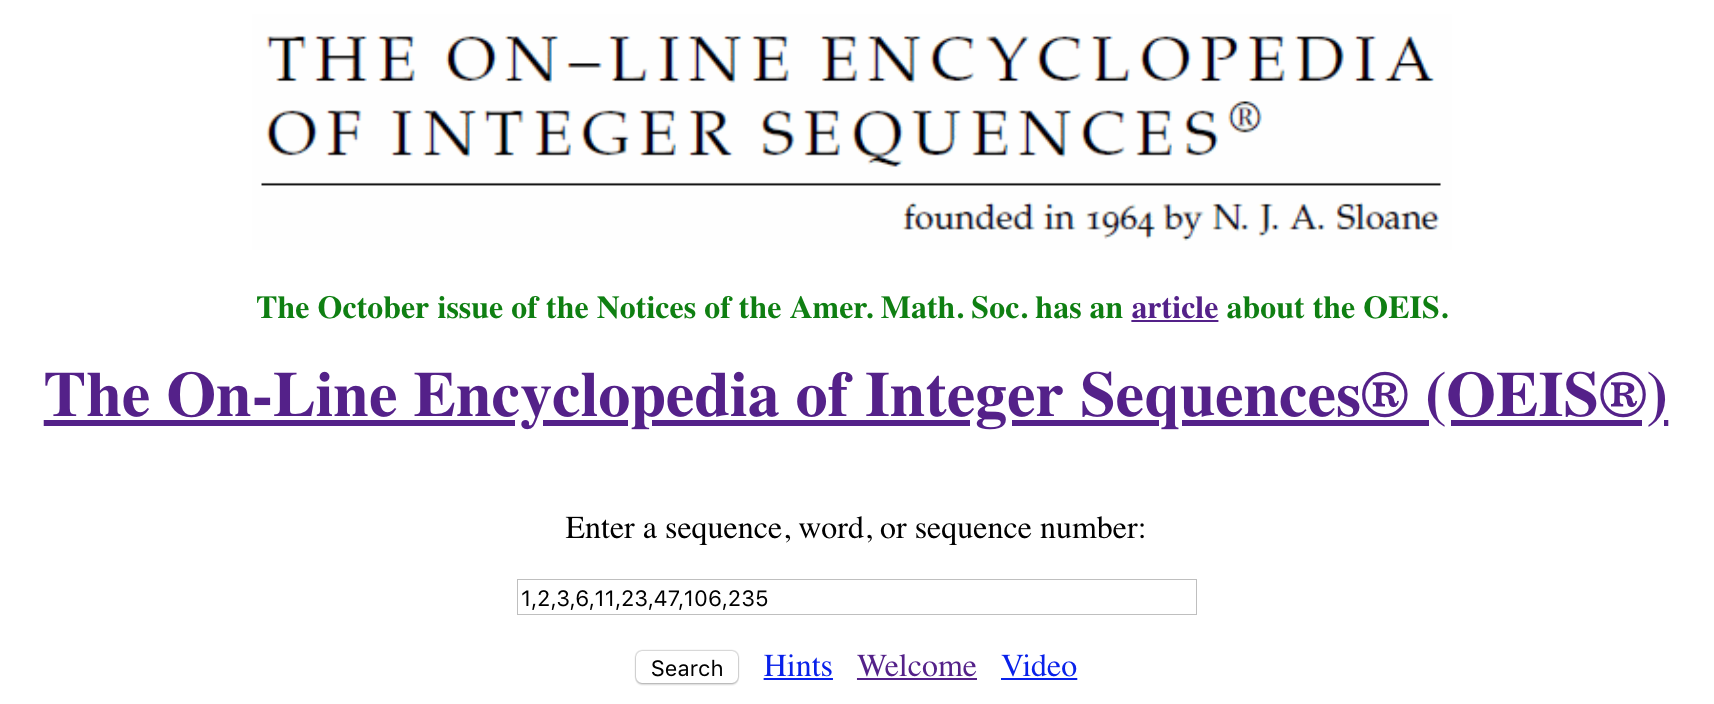
\includegraphics{deps/oeis-tools/doc/OEIS/oeis-page}
\caption{The OEIS search page and results for a query concerning the sequence
$(0,1,1,2,3,5,8,13,21,34)$.}
\label{fig:oeis:page}
\end{figure}

A similar approach in the recent literature is \citep{Nguyen_miningthe} that
mines the OEIS for new mathematical identities, discussing how to store,
compare and match integer sequences toward the formalization of some
conjectures; on the other hand, searching the word "\textit{oeis}" in GitHub
returns one hundred repositories, the majority of them (i)~host simple
implementations of scripts that download data about a desired sequence
targeting all major programming languages. Moreover, \citep{weidmann:sequencer}
is a project that tries to deduce closed formulae that generates a given list
of numbers.

Our approach complements the existing ones by providing a \textit{recursive}
and \textit{asynchronous} fetching process, vanilla data storage in JSON files
and visualization of relations among sequences; the description of each tool is
addressed in the following sections, respectively.

The present suite of tools had been shown at an open school on Combinatorial
Method in the analysis of Algorithms and Data Structures in Korea
\citep{Nocentini:korea}; moreover, all the sources that implements the
applications can be found online in the repository
\url{https://github.com/massimo-nocentini/oeis-tools}.

\section{The Crawler}

The script \verb|crawling.py| implements a bot that given a sequence identifier
in the form $Axxxxxx$, where $x$s are digits, it issues an HTTP request to the
main OEIS server and waits for a response; once it is received, the bot stores
data locally and, looking into the response's \verb|xref| section that contains a
set of other sequences identifiers, repeats its behaviour on each one of them,
recursively.  Such a bot is commonly known as \emph{crawler}.

Our implementation features neither threads nor race conditions nor data sync;
on the contrary, it targets \textit{pure asynchronous computation} by using
\textit{async/await} Python primitives only. The approach is educational and we
strive to create a simple but elegant codebase which boils down to $300$ lines
of Python code; eventually, it allows us to cache portions of the OEIS to speed
up repeated lookups and to restart the fetching process from the cache already
downloaded.

The script presents a help message to explain itself:
\VerbatimInput[baselinestretch=0.8]{deps/oeis-tools/doc/OEIS/crawler-help.txt}

\begin{example}
We illustrate a typical session where we start from scratch. First of all, we
want to download the OEIS content about two important and nice sequences,
namely those corresponding to the Fibonacci and Catalan numbers, respectively
identified by labels $A000045$ and $A000108$:
\VerbatimInput[baselinestretch=0.8]{deps/oeis-tools/doc/OEIS/crawler-fetching-command.txt}
After stopping the crawler, we check the content of the cache with the commands
\VerbatimInput[baselinestretch=0.8]{deps/oeis-tools/doc/OEIS/crawler-status.txt} 
which tell us that $30$ sequences had been fetched and stored in the default
directory \verb|./fetched/|.  Moreover, we can restart the crawler from where
it was interrupted with the command
\VerbatimInput[baselinestretch=0.8]{deps/oeis-tools/doc/OEIS/crawler-restarting.txt}
and we check that new sequences are actually collected,
\begin{Verbatim}[baselinestretch=0.8]
$ python3.6 crawling.py
50 sequences in cache ./fetched/
354 sequences in fringe for restarting
\end{Verbatim}
as desired.
\end{example}

Having contents stored in JSON files, whose structure is presented in Figure
\ref{fig:json-structure}, allows us to inspect and manipulate them using every
tool available in our working environment, as the next example shows.

\begin{example}
Combining the \verb|cat| command with the Python module \verb|json.tool|, that
prints JSON files with respect to indentation, we can visualize data about the
sequence of Fibonacci numbers as follows
\VerbatimInput[baselinestretch=0.8]{deps/oeis-tools/doc/OEIS/crawler-A000045-chunk.txt}
\end{example}

\begin{figure}
\includegraphics{deps/oeis-tools/doc/OEIS/json-structure}
\caption{The complete structure of the JSON encoding of OEIS content about the
sequence $A000045$; in particular, the property \texttt{xref}, highlighted in
\textcolor{blue}{blue}, is left expanded because of its importance in the
recursive behaviour of the crawler, namely every label in this section bacomes
a candidate sequence for the fetching process.}
\label{fig:json-structure}
\end{figure}

Our implementation takes strong inspiration from
\citep{VANROSSUM:DAVIS:async:await} and provides the following abstractions:

\begin{description}

\item[\texttt{reader}] objects, that have the responsibility to be
\textit{asynchronous iterators} in the sense that they have to respond to the
message \verb|__anext__|, where the computation waits asynchronously for
incoming data from the \verb|self.read| coroutine. The following code
implements the description precisely,
\inputminted[stripnl=false,firstline=28,lastline=39,baselinestretch=0.8]
{python}{deps/oeis-tools/src/crawling.py} 

\item[\texttt{fetcher}] objects have the responsibilities (i)~to create a socket with
OEIS server, (ii)~to establish a working connection, (iii)~to send an HTTP \verb|GET|
request for the desired sequence, (iv)~to wait for the fetching process completes
and (v)~to close the socket and signal that the it ends successfully.
A literal translation follows,
\inputminted[stripnl=false,firstline=41,lastline=86,baselinestretch=0.8]
    {python}{deps/oeis-tools/src/crawling.py}

\item[\texttt{crawler}] objects have the responsibilities (i)~to keep a queue of task,
one for each candidate sequence, (ii)~to put each ready task into the
scheduling process and (iii)~to reclaim memory for the completed ones and
(iv)~to deque them, eventually; again, its code follows
\inputminted[stripnl=false,firstline=89,lastline=117,baselinestretch=0.8]
    {python}{deps/oeis-tools/src/crawling.py}

\end{description}

\iffalse
Finally, the function \verb|oeis| puts all together and it is the main
interface exported by the \verb|crawling| module:
\inputminted[stripnl=false,firstline=195,lastline=221,baselinestretch=0.8]
    {python}{deps/oeis-tools/src/crawling.py}
\fi

\section{The (Pretty) Printer}

The script \verb|pprinting.py| provides a proxy for searching into the OEIS,
therefore it shows exactly the same contents you see from usual web interface
on \url{http://oeis.org}; additionally, it provides (i)~tabular representations
of \verb|data| sections in \textit{one} and \textit{two} dimensions using
\textit{list} and \textit{matrix} notations, respectively, (ii)~filtering
capabilities on most response's sections and (iii)~interoperability with the
crawler tool by taking advantage of cached sequences.

The script presents a help message to explain itself:
\VerbatimInput[baselinestretch=0.8]{deps/oeis-tools/doc/OEIS/pprinting-help.txt} In the next examples
we show how \verb|pprinting|'s facilities can be used to apply filters, to
print data-only visualization and to search by an open query, respectively.

\begin{example} Typing the following command into a shell, it outputs
on the \verb|stdout| the pretty-printed contents about the sequence of
Fibonacci numbers, with two filters applied that show comments made by
prof. Barry and the first $5$ formulae only,
\VerbatimInput[baselinestretch=0.8]{deps/oeis-tools/doc/OEIS/pprinting-A000045.txt}
other sections, such as \verb|reference| and \verb|link|, are hidden by
default to provide a cleaner output.
\end{example}

\begin{example}
The following command pretty prints (i)~the first 3 sequences from our current
cache --the result may vary if you try on your own machine--, (ii)~ranking them
according to the most recent access time, (iii)~reporting data only and
(iv)~limiting up to $10$ coefficients for linear sequences:
\VerbatimInput[baselinestretch=0.8]{deps/oeis-tools/doc/OEIS/pprinting-data-only.txt}
\end{example}

\begin{example}
The following command pretty prints the responses about the \textit{open query}
"\verb|pascal triangle|", using $2$-dimension representation for matrices
in \verb|data| sections, and reports the first $2$ sequences only,
\VerbatimInput[baselinestretch=0.8]{deps/oeis-tools/doc/OEIS/pprinting-pascal-matrix.txt}
\end{example}

In parallel of the terminal interface, we develop pretty printing functions
that integrates in Jupyter notebooks. The aim remains the same, namely to
present contents taken from the OEIS targeting a different environment that
accepts their representation; this is the time of a dynamic web interface that
allows us to evaluate Python code on the fly. Using the Markdown language
(\url{https://daringfireball.net/projects/markdown/}) to write textual content,
we propose another view of the same data, as shown in Figures
\ref{fig:oeis:notebook:fibonacci}, \ref{fig:oeis:notebook:catalan} and
\ref{fig:oeis:notebook:pascal}; in particular, we take advantage of
(i)~hyper-references to make labels of sequences clickable to quickly visit
them, (ii)~font styles to emphasize words in italics and bold-face and (iii)~to
render math expressions properly, such as $2$-dimensional array representation
for matrices.

\begin{figure}
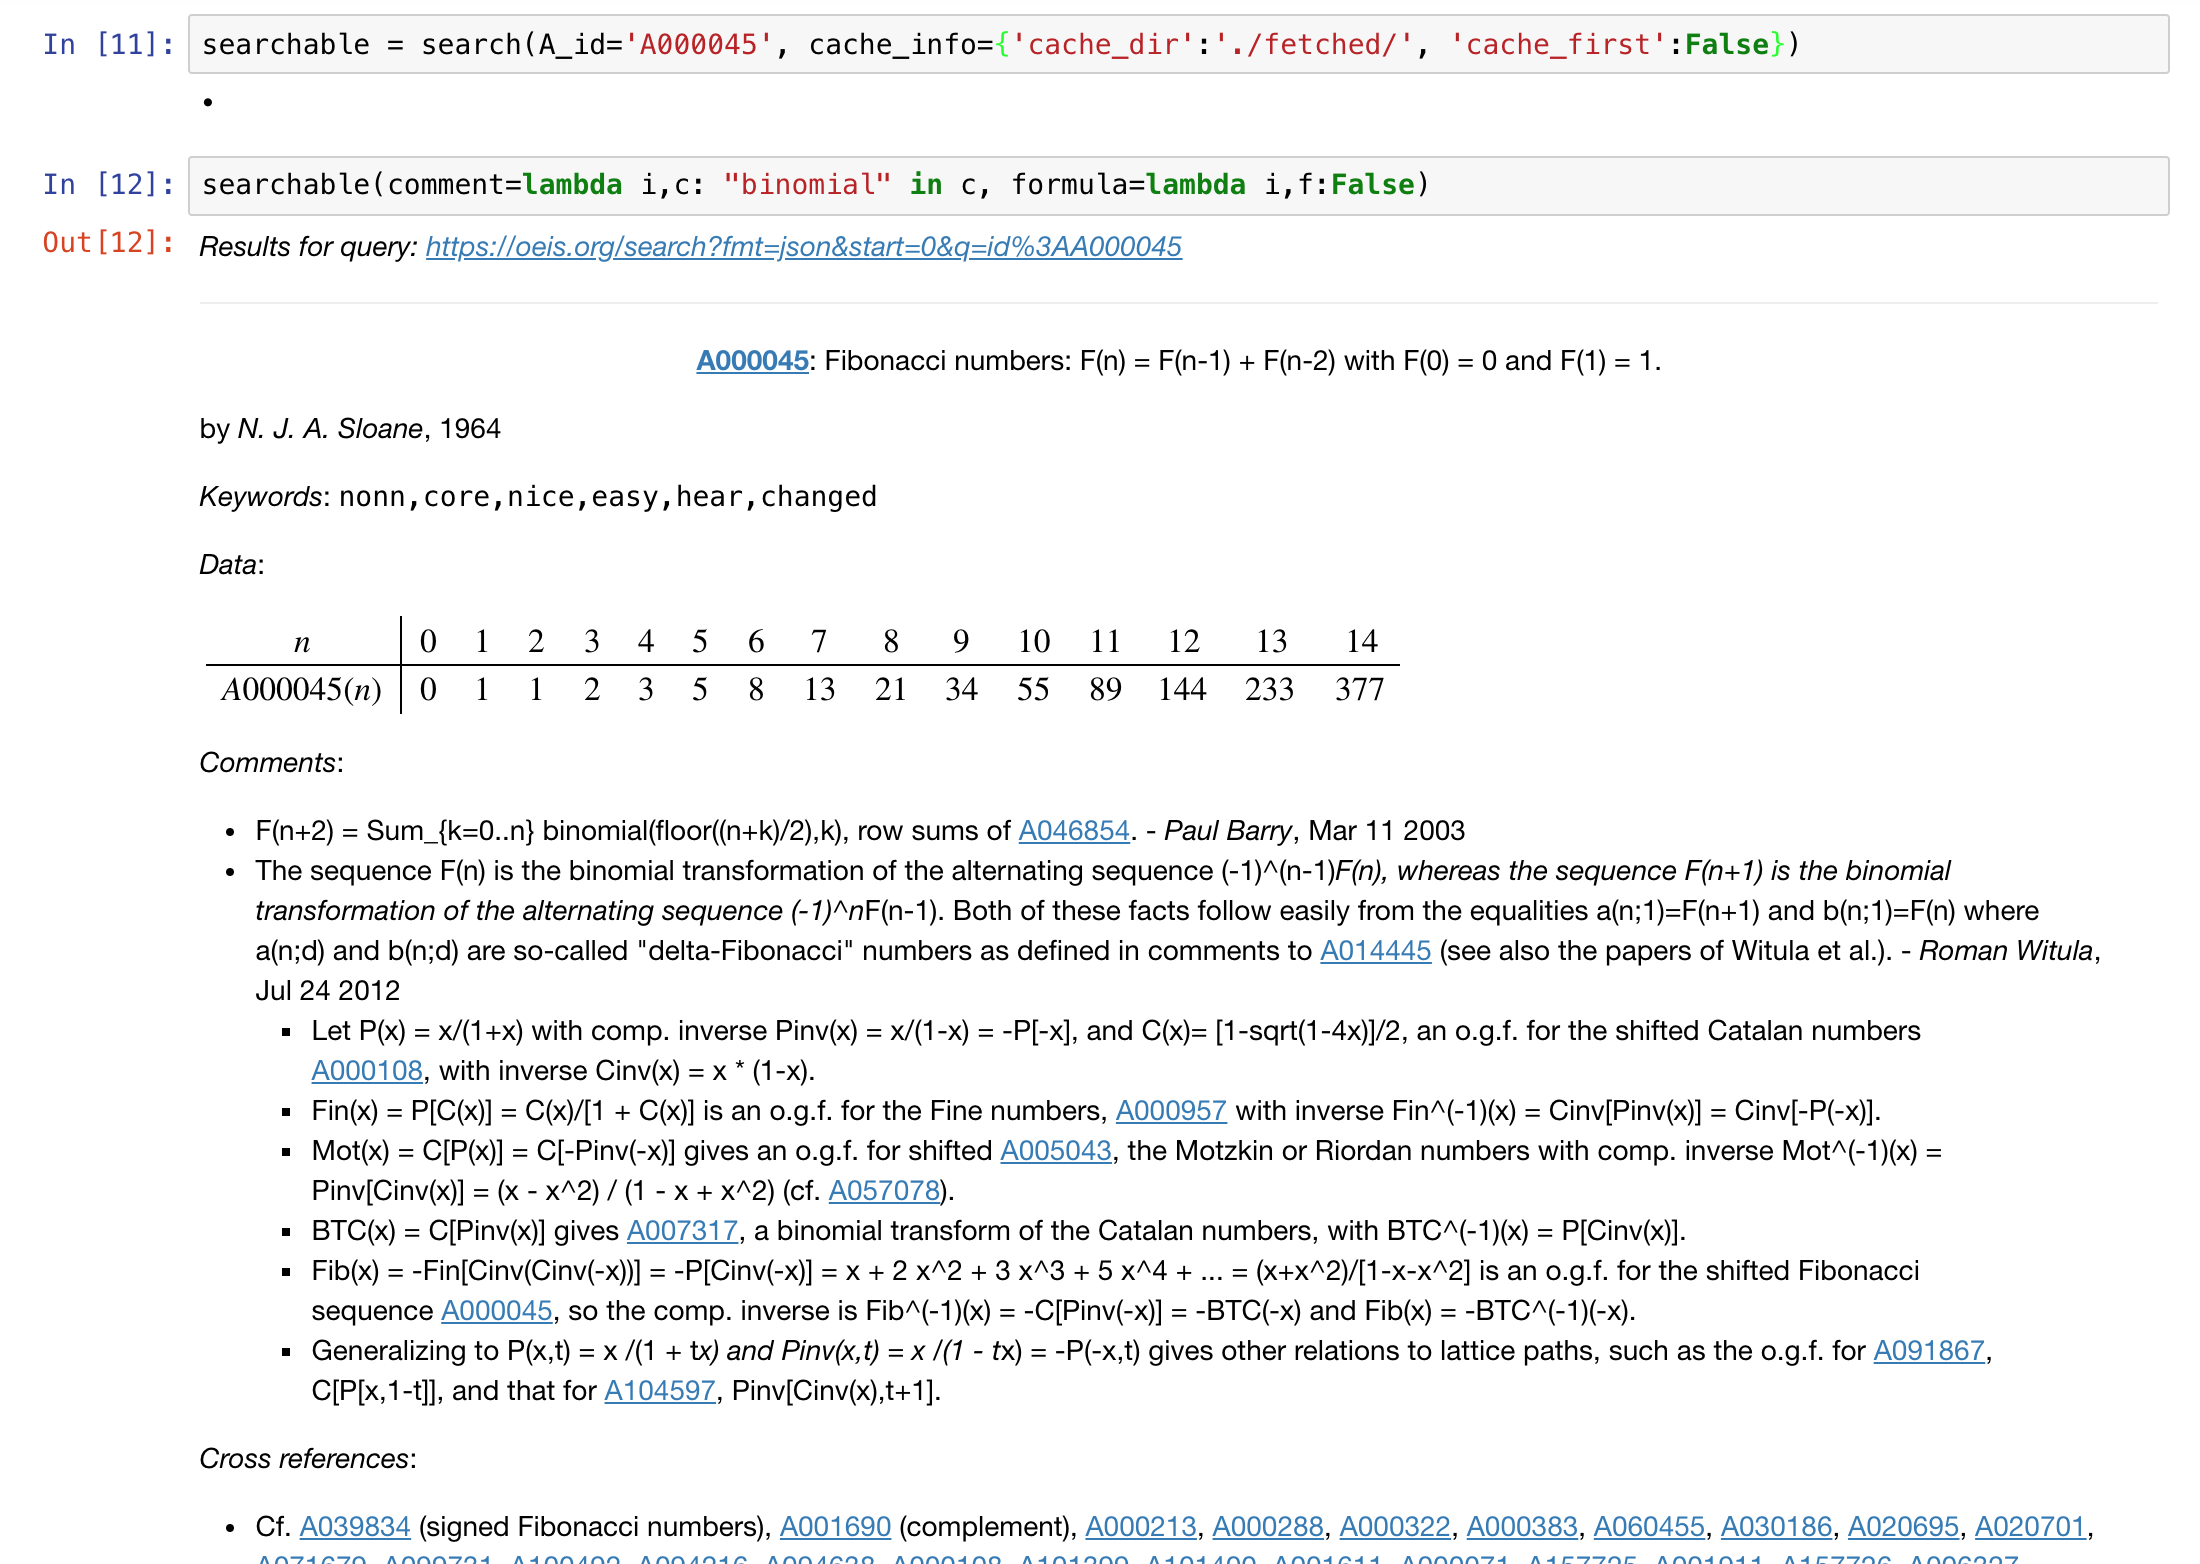
\includegraphics[width=.7\pagewidth]{deps/oeis-tools/doc/OEIS/notebook-fibonacci}
\caption[][10.5cm]{This screenshot shows search results about the Fibonacci numbers where
(i)~the section about comments is filtered such that the word "\emph{binomial}"
has to appear in their text and (ii)~the section about formulae is hidden.}
\label{fig:oeis:notebook:fibonacci}
\end{figure}

\begin{figure}
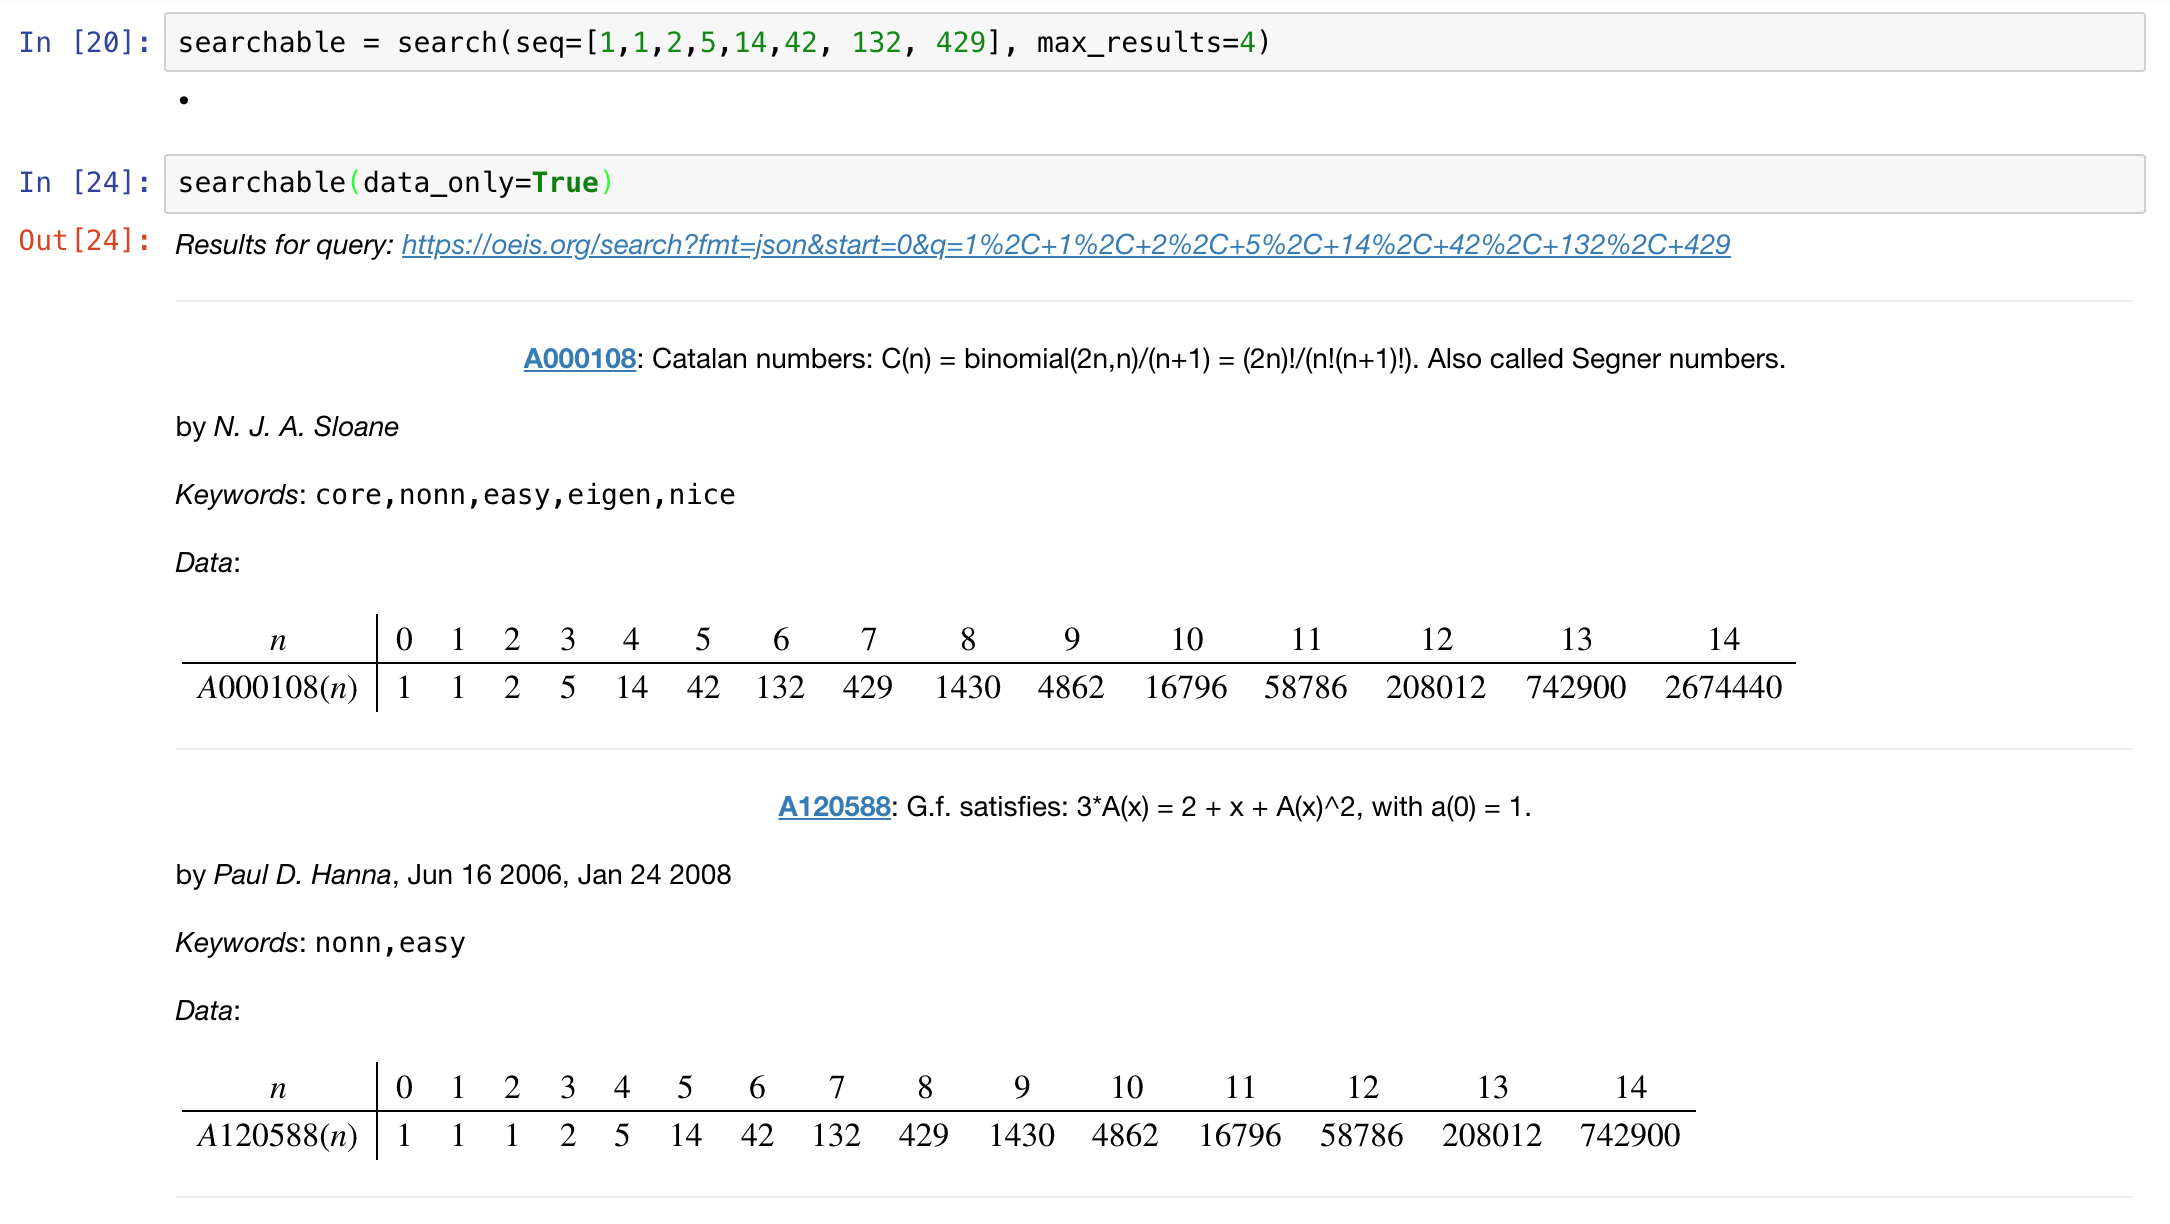
\includegraphics[width=.7\pagewidth]{deps/oeis-tools/doc/OEIS/notebook-catalan}
\caption[][8.5cm]{This screenshot shows search results of a query using a subsequence,
showing \emph{data} sections only.}
\label{fig:oeis:notebook:catalan}
\end{figure}

\begin{figure}
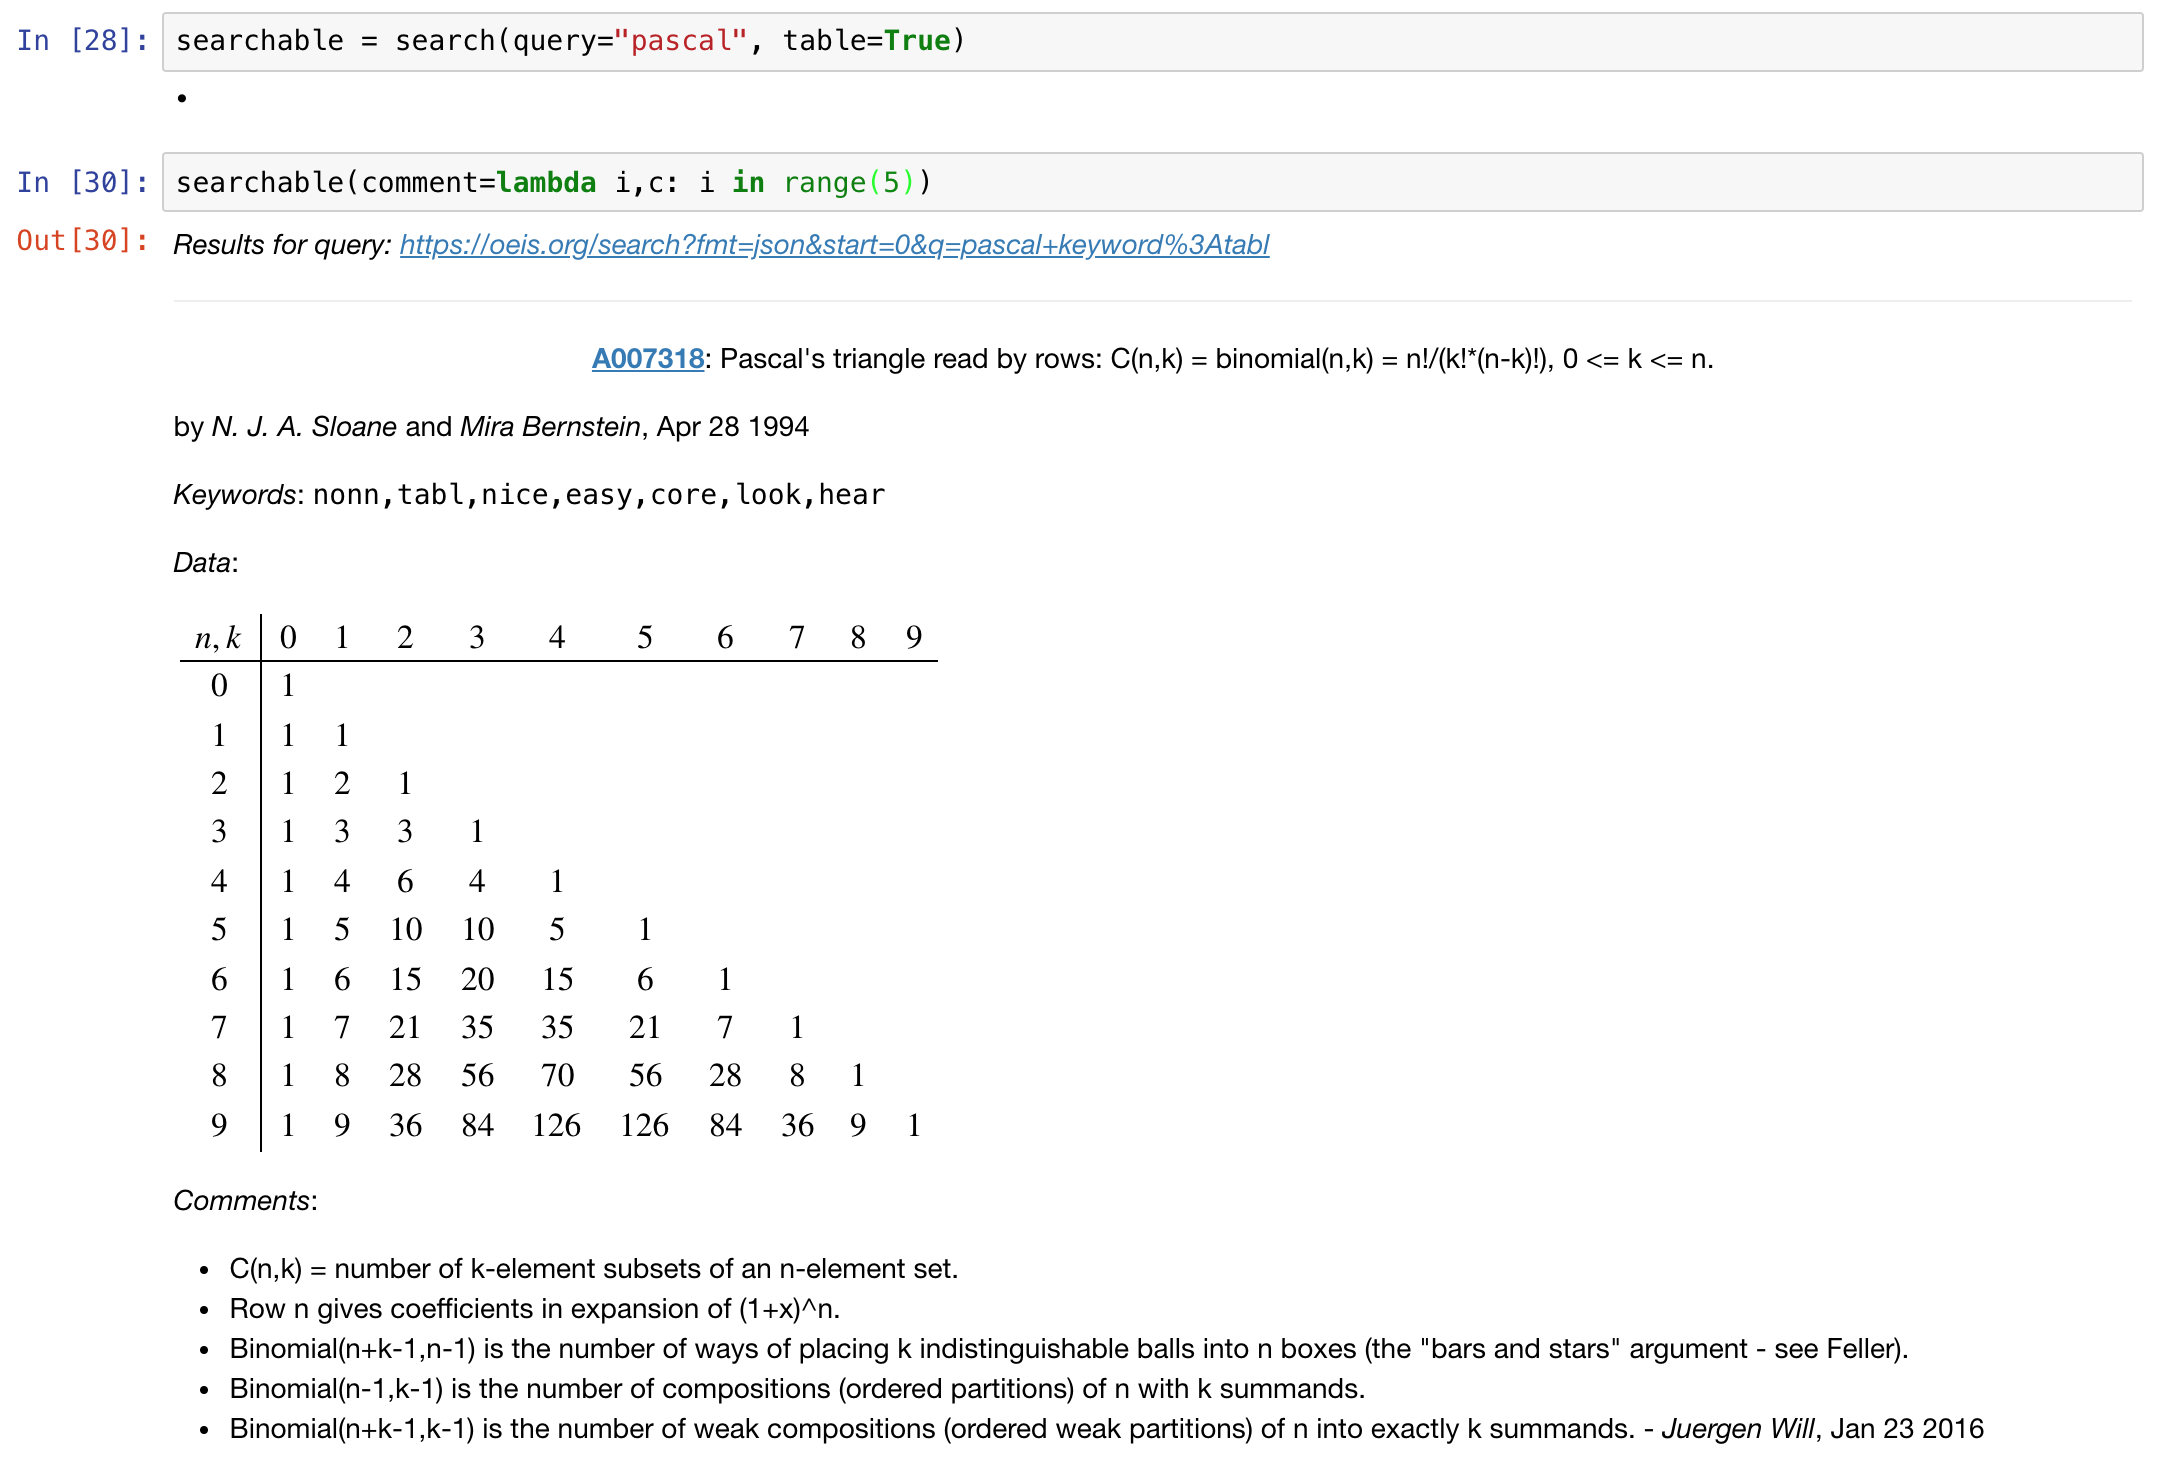
\includegraphics[width=.7\pagewidth]{deps/oeis-tools/doc/OEIS/notebook-pascal}
\caption[][10cm]{This screenshot shows search results of an open query using the
"\emph{pascal}" keyword, representing the \emph{data} section as a
$2$-dimensional array.  }
\label{fig:oeis:notebook:pascal}
\end{figure}

\section{The Grapher}

The script \verb|graphing.py| allows us to represent networks where vertices
are sequences and edges are connections among them, according to \verb|xref|
sections in their JSON encodings. It integrates with the crawler tool by
parsing the fetched files and creates \verb|Graph| objects, defined in the
Python module \verb|networkx|, having different layouts according to a set of
drawing algorithms.

It presents a help message to explain itself:
\VerbatimInput[baselinestretch=0.8]{deps/oeis-tools/doc/OEIS/graphing-help.txt}

\begin{example}
The following command draws the graph shown in Figure
\ref{fig:oeis:sequences:network}, where the width of each vertex grows
according to the number of its \textit{incoming} connections,
\begin{Verbatim}[baselinestretch=0.8]
$ python3.6 graphing.py --layout FRUCHTERMAN-REINGOLD graph.png
\end{Verbatim}
in order to emphasize most referenced sequences.
\end{example}

\begin{figure}
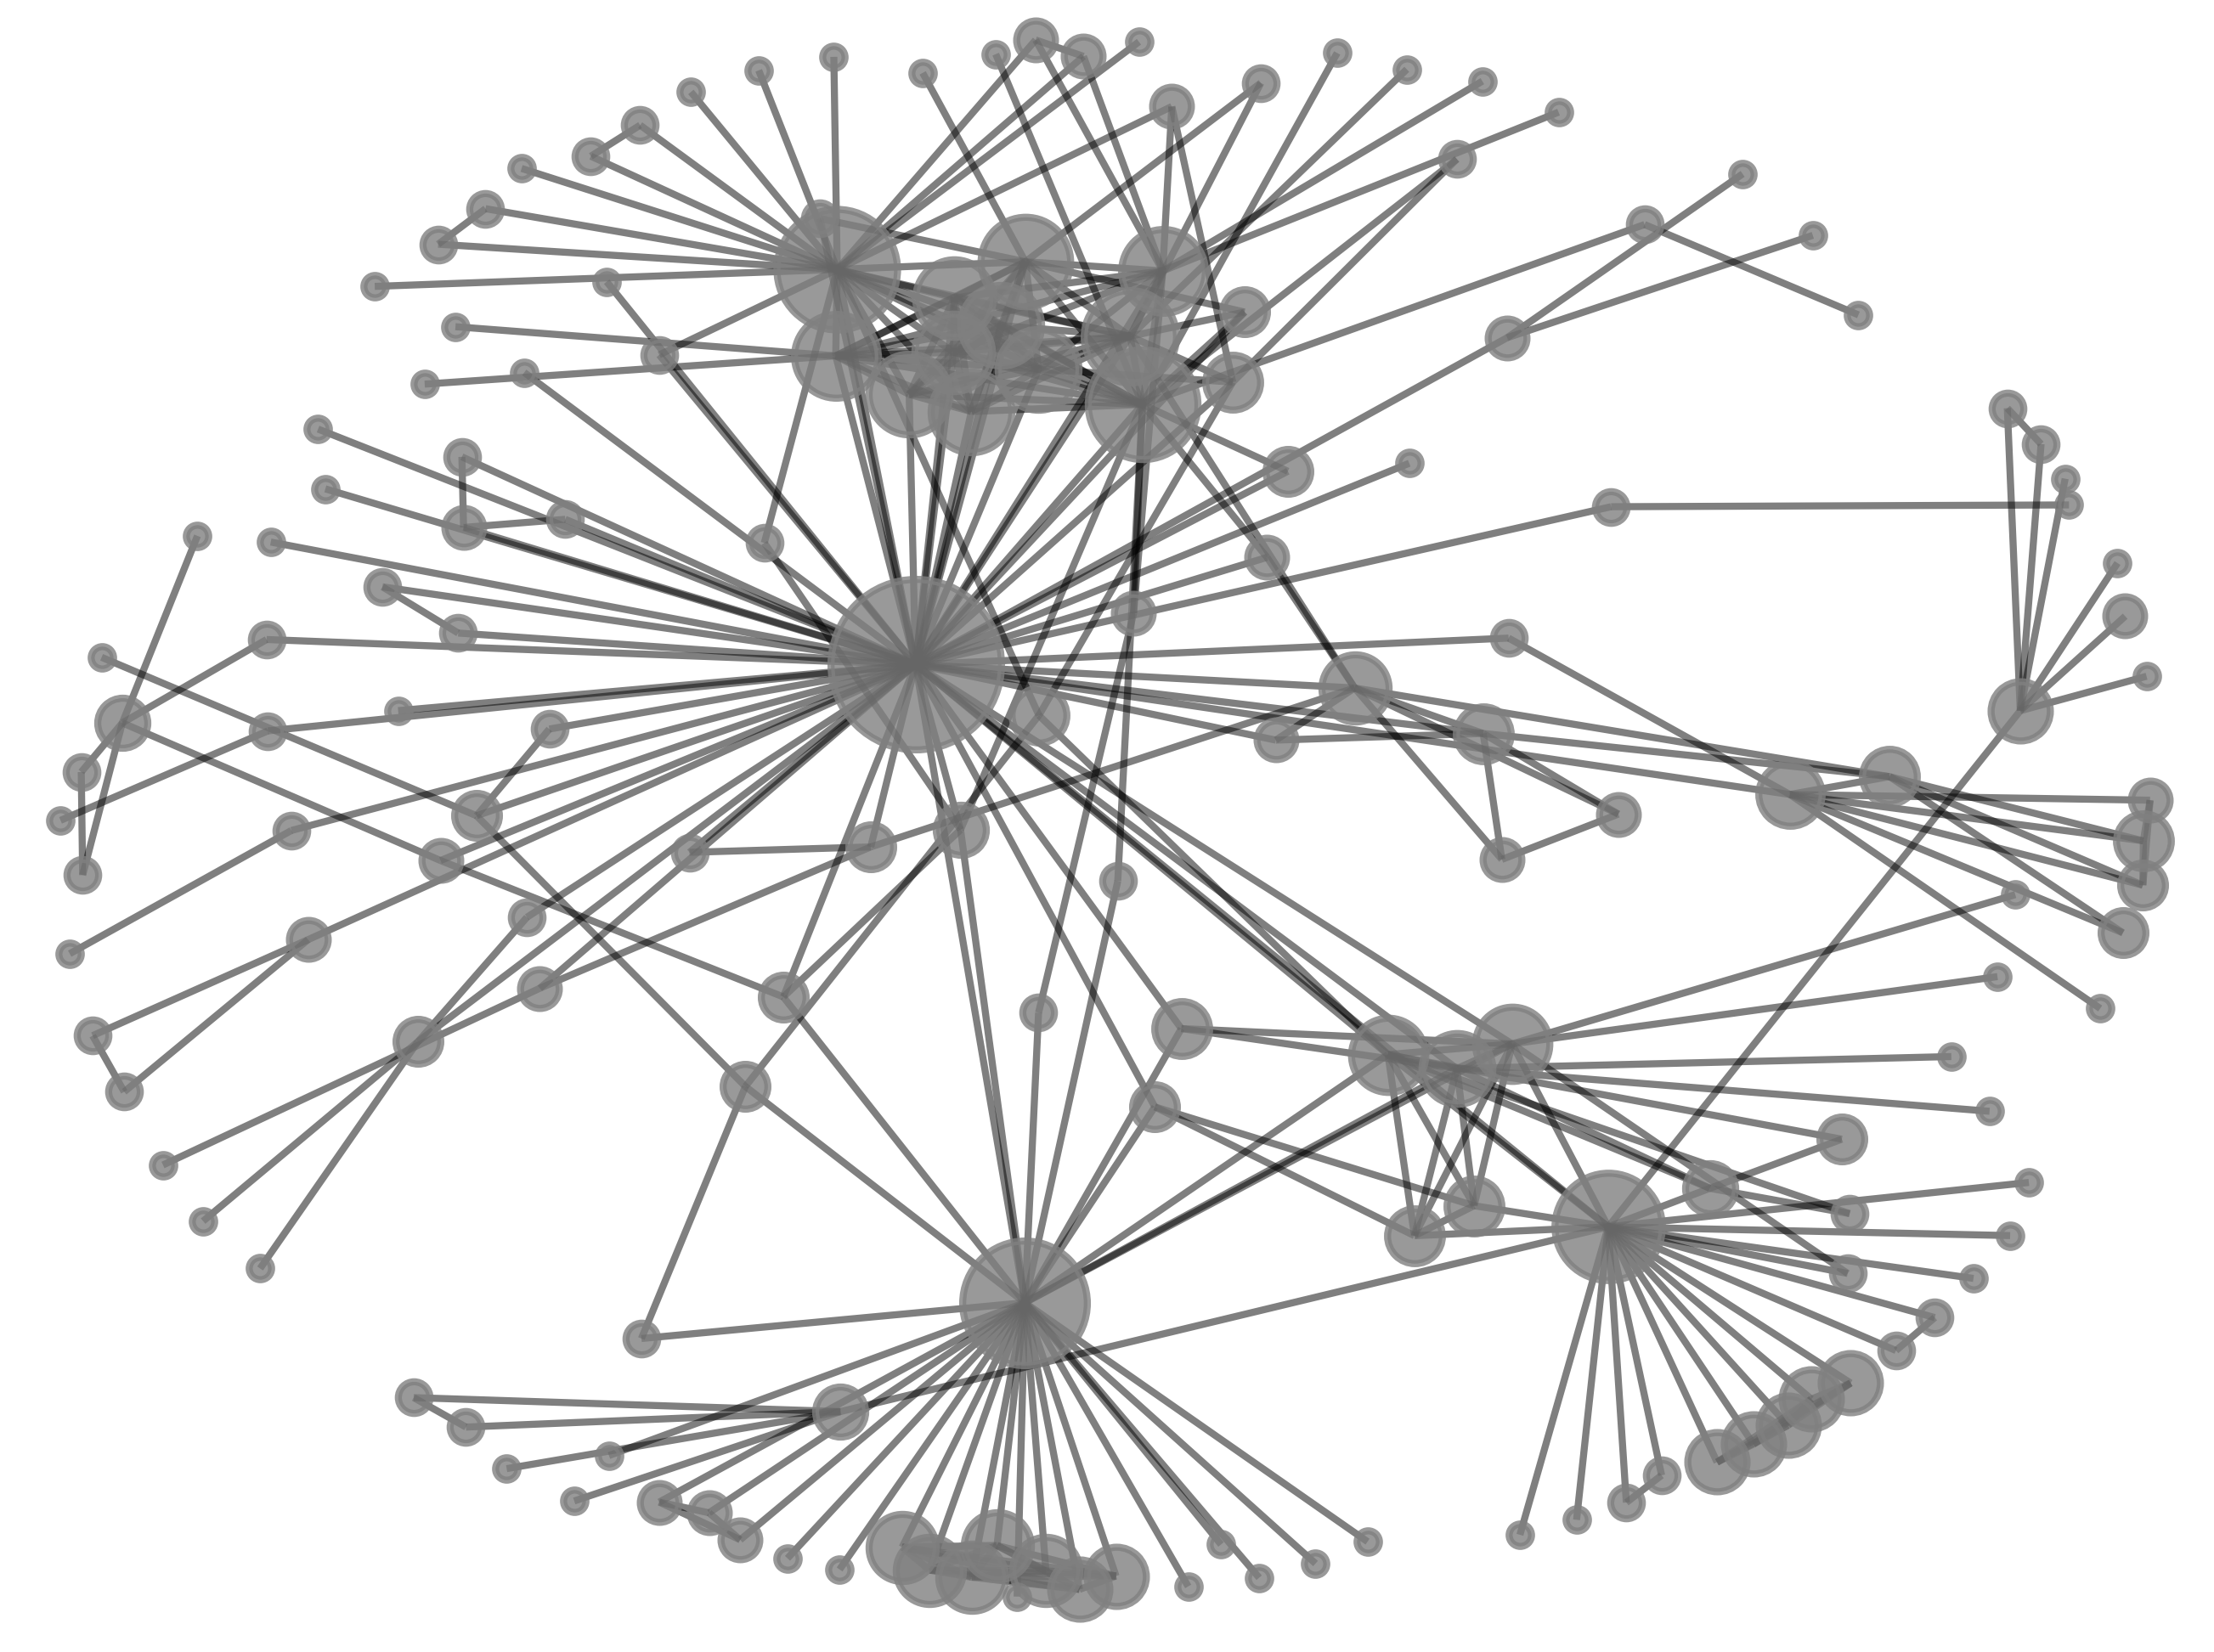
\includegraphics{deps/oeis-tools/doc/OEIS/graph1}
\caption{Sequences network where vertices are emphasized according to the
number of incoming connections.}
\label{fig:oeis:sequences:network}
\end{figure}

Moreover, it can extract essential data from the whole set of JSON files, such
as the list of vertices and edges, to interface with third-party software tools
that provide different visualizations; in particular, libraries using the
\textit{Javascript} programming language are very powerful and the output they
produce are very expressive. For our purposes, we use the \verb|arborjs|
library (freely available at \url{http://arborjs.org/}) to display two
additional graphs described in the next two examples, respectively.

\begin{example}
Figure \ref{fig:oeis:sequences:network:fibonacci:catalan} reports a new
unlabeled graph that shows the underlying structure of sequences connections.
Here, the layout spreads vertices such that the ones having many
\textit{outgoing} connections are centered, while those having poor
connectivity are left on borders.

Under the hood, the Fibonacci and Catalan numbers are the two central sequences
and both of them have an orbit which contains a set of highly connected
sequences.
\end{example}

\begin{figure}
%\begin{sideways}
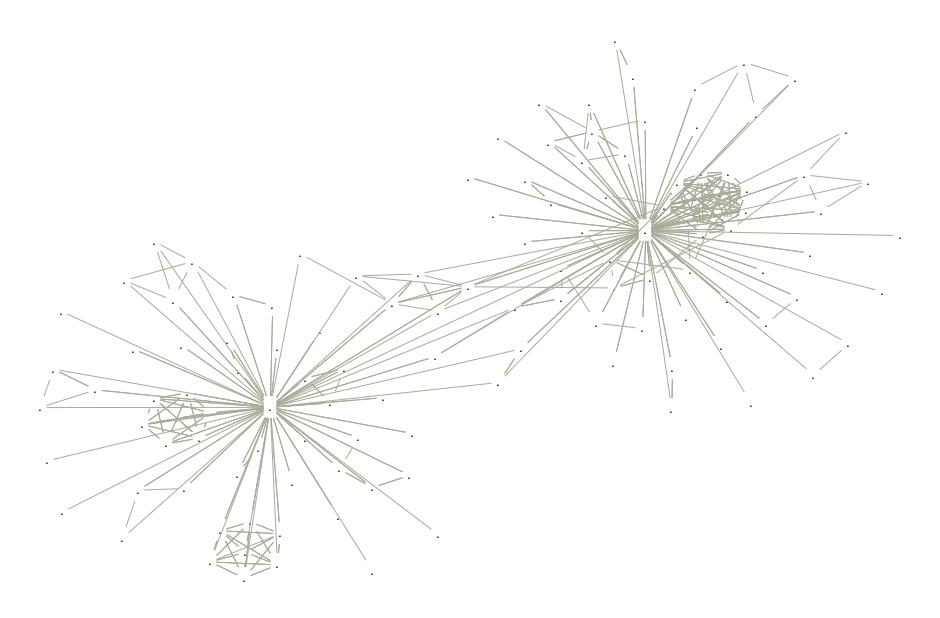
\includegraphics[width=15cm, height=15cm]{deps/oeis-tools/doc/OEIS/points}
\caption[][8cm]{Sequences network abstracting over identifier to spot the underlying
structure.}
%\end{sideways}
\label{fig:oeis:sequences:network:fibonacci:catalan}
\end{figure}

\begin{example}
On the other hand, Figure
\ref{fig:oeis:sequences:network:fibonacci:catalan:labeled} adds labels and
colors to vertices in order to spot their identity and their relevance
according to a combination of their properties. In particular, each color is
represented by an RGB tuple that gets weigths (i)~the number of comments and
formulae for \textit{red}, (ii)~the number of references and links for
\textit{green} and (iii)~the number of incoming and outgoing connections for
\textit{blue}, respectively. Moreover, we get the complement to $255$ of each
component because many sequences have not so many details and this manipulation
allows us to obtain cleaner and more expressive graphs.

For the sake of clarity, the two sequences in evidence are the Fibonacci and
Catalan numbers, the former has the color $(006100)_{16}$ and its complement
$(FFFFFF)_{16}-(006100)_{16}=(FF9EFF)_{16}$ means that it has many comments,
formulae and connections; the latter has the color $(7C00E5)_{16}$ and its
complement $(FFFFFF)_{16}-(7C00E5)_{16}=(83FF1A)_{16}$ means that it has lots
of comments, links and references.
\end{example}

\begin{remark}
Recall that the interpretations given in the previous examples concern a
\textit{subset} of the OEIS only, in particular the one fetched in our session;
finally, the more we crawl, the more graphs are effective and accurate.
\end{remark}

\begin{figure}
\begin{sideways}
%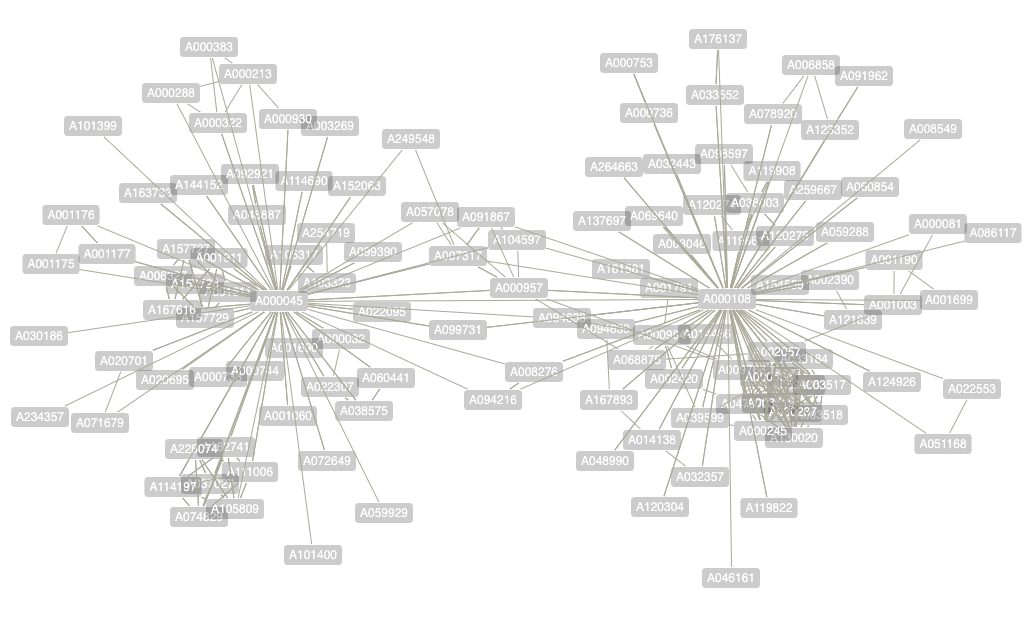
\includegraphics[width=20cm, height=20cm]{deps/oeis-tools/doc/OEIS/labels}
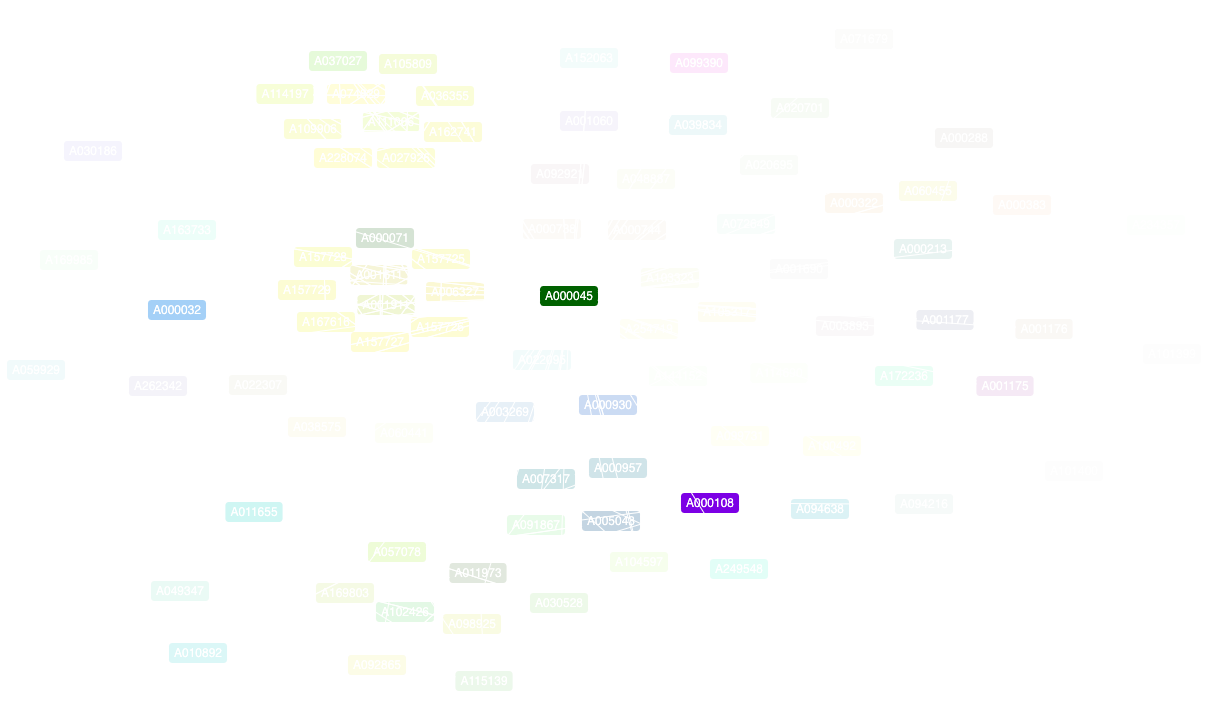
\includegraphics[width=25cm, height=25cm]{deps/oeis-tools/doc/OEIS/coloured}
\caption{Sequences network with labelel vertices, here we see that the sequence
of \textit{Fibonacci numbers} (\url{https://oeis.org/A000045}) and of
\textit{Catalan numbers} (\url{https://oeis.org/A000108}) are the two central
sequences, respectively.}
\end{sideways}
\label{fig:oeis:sequences:network:fibonacci:catalan:labeled}
\end{figure}

\begin{example}
Finally, crawling for a while to get more sequences, we represent their
connections in Figure
\ref{fig:oeis:sequences:network:fibonacci:catalan:circular}, arranging them
using a circular layout and we emphasize vertices in the \textit{dominating
set} using the \textit{red} color.
\end{example}

\begin{figure}
\hspace{-3cm}
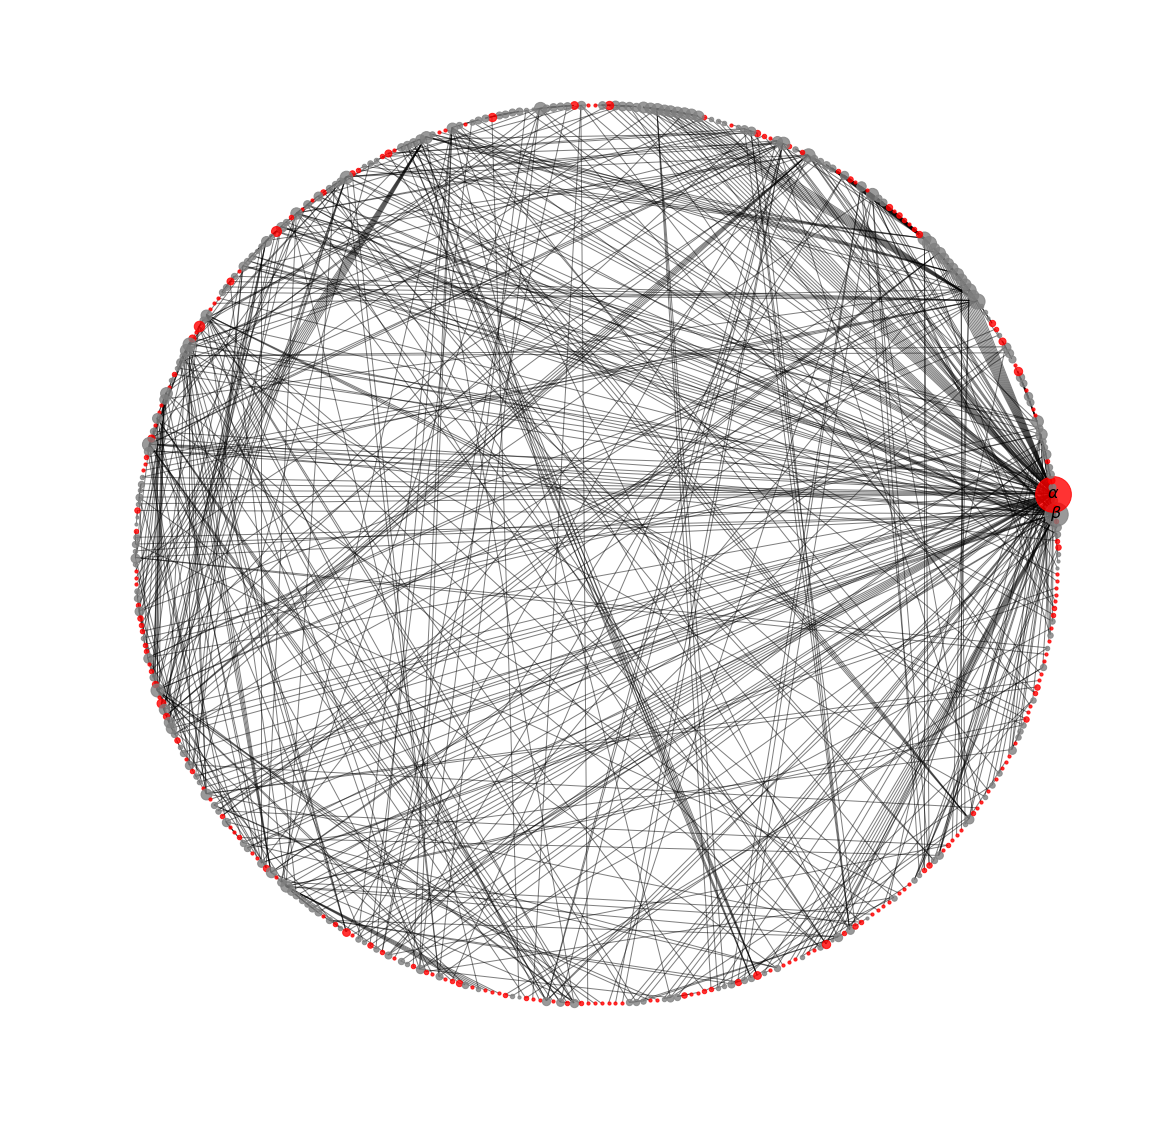
\includegraphics[width=20cm, height=20cm]{deps/oeis-tools/doc/OEIS/circular}
\caption{A bigger sequences network composed of $419$ sequences; here the
sequence of \textit{Fibonacci numbers} is denoted by $\alpha$ and the sequence
of \textit{Catalan numbers} is denoted by $\beta$, respectively.}
\label{fig:oeis:sequences:network:fibonacci:catalan:circular}
\end{figure}

\section*{Conclusions}

This chapter presents a suite of tools that interacts with the \textit{Online
Encyclopedia of Integer Sequences}, whose primary goal is to automate simple
and repetitive operations such as (i)~crawling sequences to hold a local copy
stored in JSON files, (ii)~pretty printing data with filtering capabilities,
both in the terminal and in Jupyter (\url{http://jupyter.org/}) notebooks and
(iii)~to visualize connections among sequences using graphs.

In parallel, this suite has been though to be open to extension
and to interface with the hosting environment, UNIX in particular. For
instance, the printer can be used in pipe with the \verb|less| command to gain
scroll and search features for free or the grapher can be augmented to generate
more detailed graph descriptions to be processed by visualization tools.

An additional work direction is to make graphs interactive, namely to tie
together the crawler and the grapher in a web-browser interface such that a
click on a vertex triggers the execution of the fetching process (unless it has
been downloaded already) and the new connections are added to the network
dynamically.




\iffalse

\begin{figure}
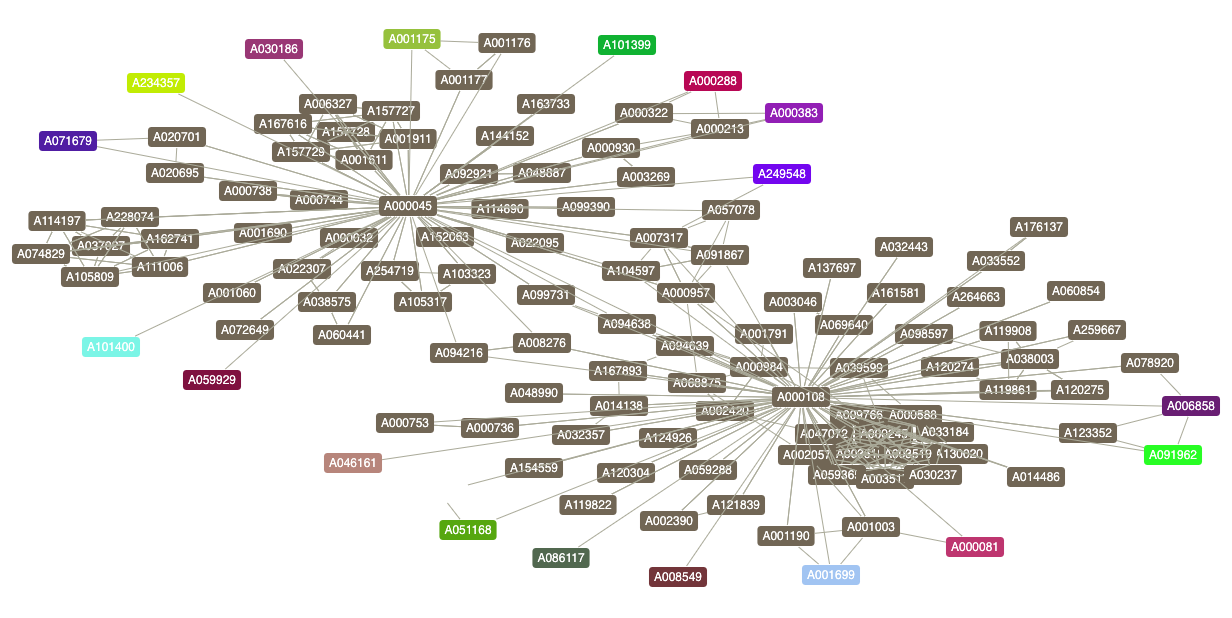
\includegraphics{deps/oeis-tools/doc/OEIS/fibonacci-catalan}
\caption{Sequences network fetched by commands issued in the discussed session.}
\label{fig:oeis:sequences:network}
\end{figure}

\notbreakable{
    \inputminted[stripnl=false,firstline=31,lastline=44]
        {python}{deps/oeis-tools/src/graphing.py}
}

\notbreakable{
    \inputminted[stripnl=false,firstline=46,lastline=76]
        {python}{deps/oeis-tools/src/graphing.py}
}

\fi
